\documentclass{scrartcl}
\usepackage{graphicx}
\usepackage{hyperref}
\usepackage{tikz}
\usepackage{xcolor}
\usepackage{amsmath}
\usepackage{float}



\usetikzlibrary{shapes}
\usetikzlibrary{positioning}





% Title Page
\title{Master Thesis}
\subtitle{A Remotely-driven Hoverboard With Platform Learning Control}

\author{Author: Esteve Tarrag\'o \\
	Advisors: Llu\'is Ros \ Enric Celaya\\
	Tutor: Merc\`e Oll\'e\\
	MSc in Advanced Mathematics and Mathematical Engineering\\
	Institut de Robòtica i Informàtica Industrial
}
\begin{document}
\maketitle

\newpage
\begin{abstract}
	TO DO: This is the abstract
\end{abstract}

\newpage
\tableofcontents

\section{Objective}
The objective of this project is to build a dynamic robot in order to experiment with reinforcement learning algorithms with real data. We wish to make this experiments easy and cheap to reproduce so we will try minimize its components and fabrication cost. 

The chosen robot is inspired in a \textit{segway hover-board}, similar to the one in Figure \ref{fig:Picture of a commercial segway hover-board}. The two wheels are controlled with classic control algorithms and the inclination of the central body is controlled with a reinforcement learning algorithm.

\begin{figure}
	\centering
	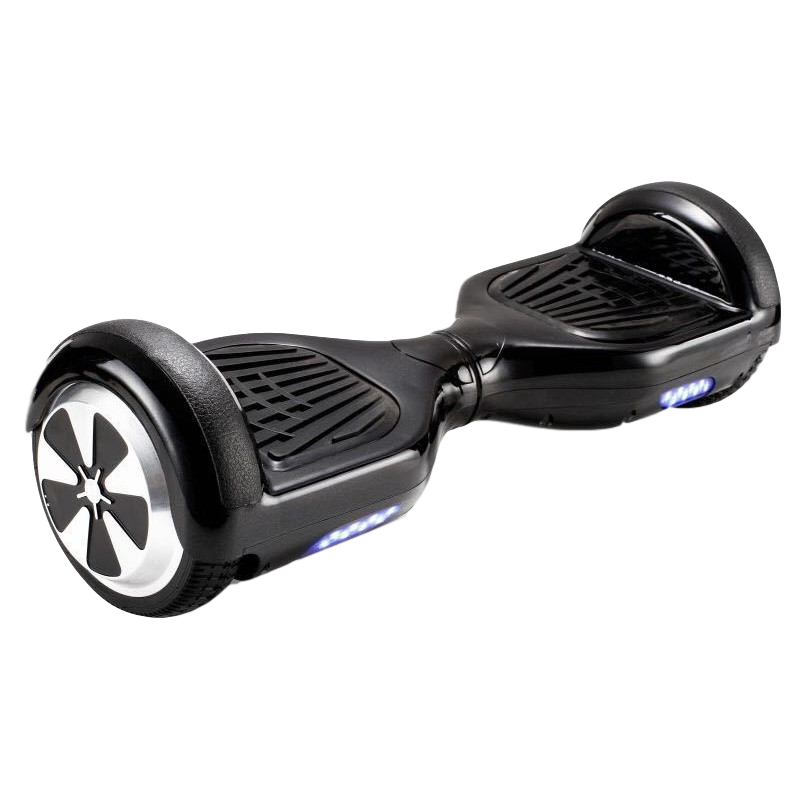
\includegraphics[width=8cm]{img/segway_hoverboard_picture.png}
	\caption{Picture of a commercial \textit{segway hover-board} }
	\label{fig:Picture of a commercial segway hover-board}
\end{figure}
\section{Initial design considerations}
The first thing we decided is the number of actuators.
Most of segway robot include two motors for the motion control but
we added a third on in order to control the inclination.
We included three motors in total because we want to control
three degrees of freedom (inclination and speed of both wheels).

In order to control the inclination of the platform we needed to produce
an external torque to the platform. We considered three methods: accelerating
a flywheel, holding a pendulum in a non-vertical position and air friction
with a fan. We discarded the last one due to the high speeds we needed to obtain
a reasonable torque on the platform.

Both methods have strengths in different situations so we decided to build a mixed
piece that could combine both. 


We took two more restriction in our design. The first one symmetry along the 
inclination axis in order to have an equilibrium in all possible inclinations
without the need of external forces. 
We also took in consideration that some experiments may start clumsy so none of
the configurations should touch the ground to avoid crashes. Figure \ref{fig:Side render view}
illustrates this last restriction.   

The design of the robot is done with the 3D design software 
\href{https://www.freecadweb.org/}{Free-cad} and most of parts where 3D printed. 3D printing has
also it's own restrictions, for example not being able to print parts bigger than 25 cm.
All part files are uploaded to the GitHub repository \url{https://github.com/tarragoesteve/TFM} under the hardware folder.

You can see the main of an initial design views on Figure \ref{fig:Isometric render view}, \ref{fig:Front render view}, \ref{fig:Top render view} and \ref{fig:Side render view}.

\begin{figure}
	\centering
	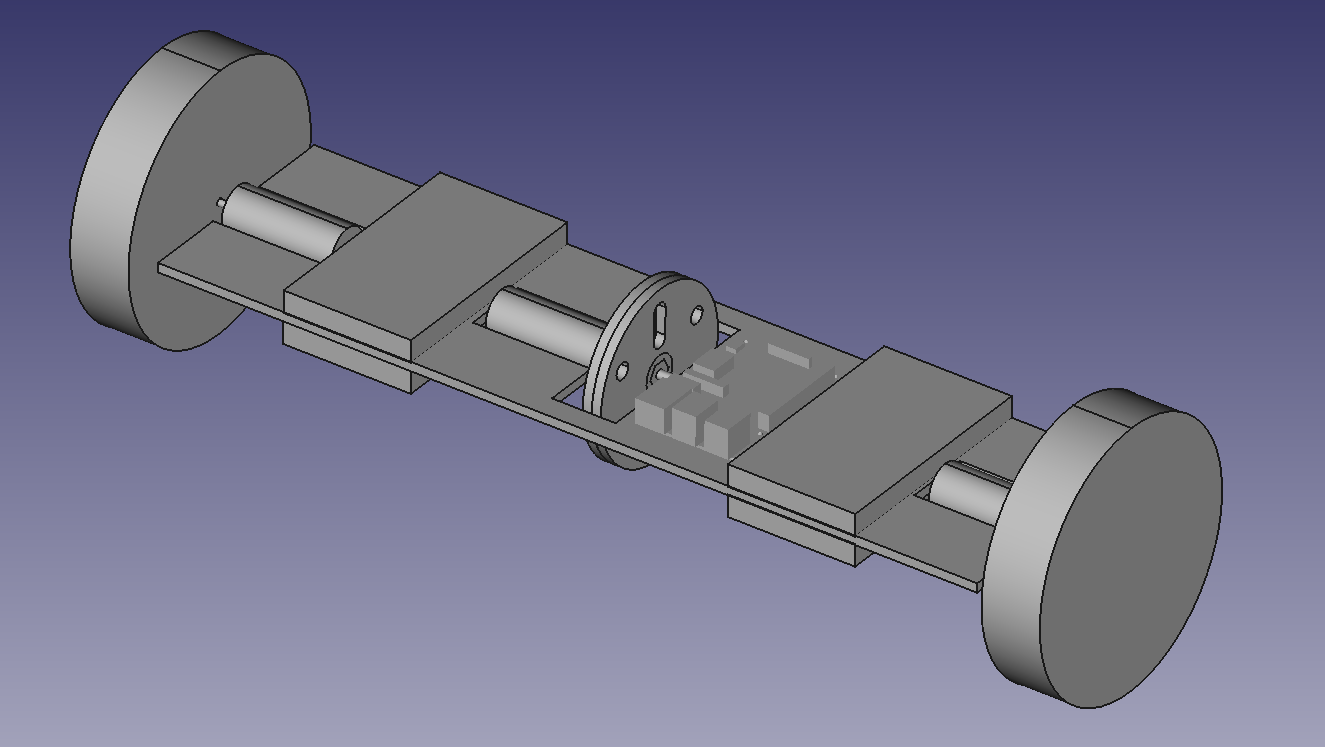
\includegraphics[width=10cm]{img/isometric_view.png}
	\caption{Isometric render view}
	\label{fig:Isometric render view}
\end{figure}
\begin{figure}
	\centering
	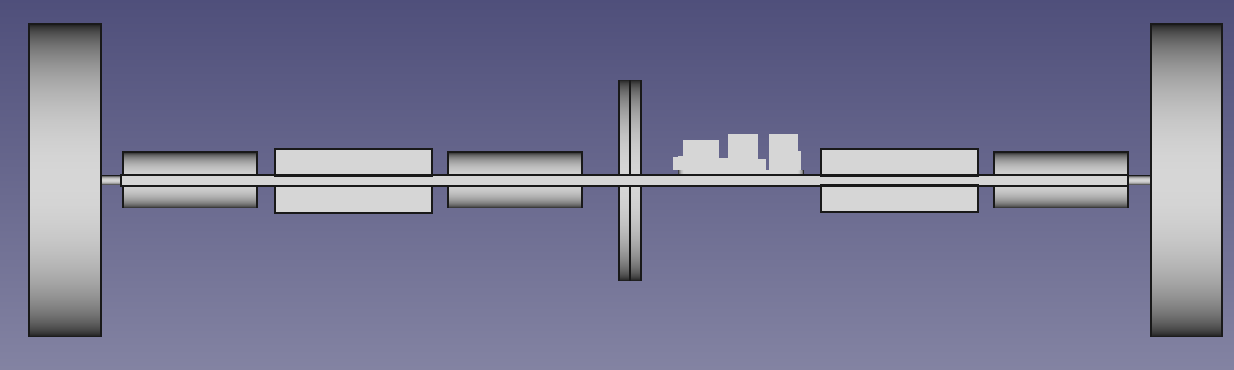
\includegraphics[width=10cm]{img/front_view.png}
	\caption{Front render view}
	\label{fig:Front render view}
\end{figure}
\begin{figure}
	\centering
	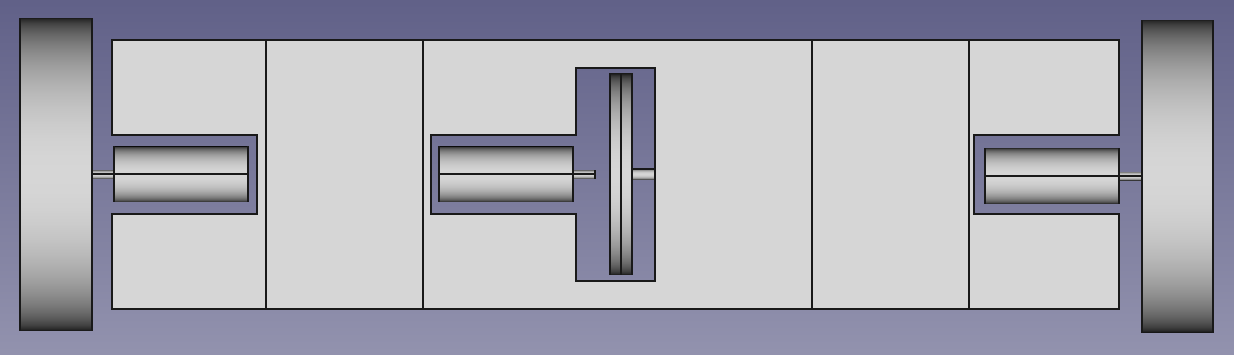
\includegraphics[width=10cm]{img/top_view.png}
	\caption{Top render view}
	\label{fig:Top render view}
\end{figure}
\begin{figure}
	\centering
	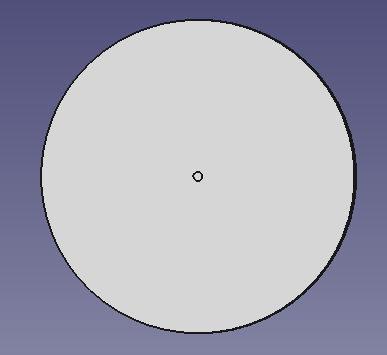
\includegraphics[width=4cm]{img/side_view.png}
	\caption{Side render view}
	\label{fig:Side render view}
\end{figure}

\subsection{Flywheel design}
\begin{figure}
	\centering
	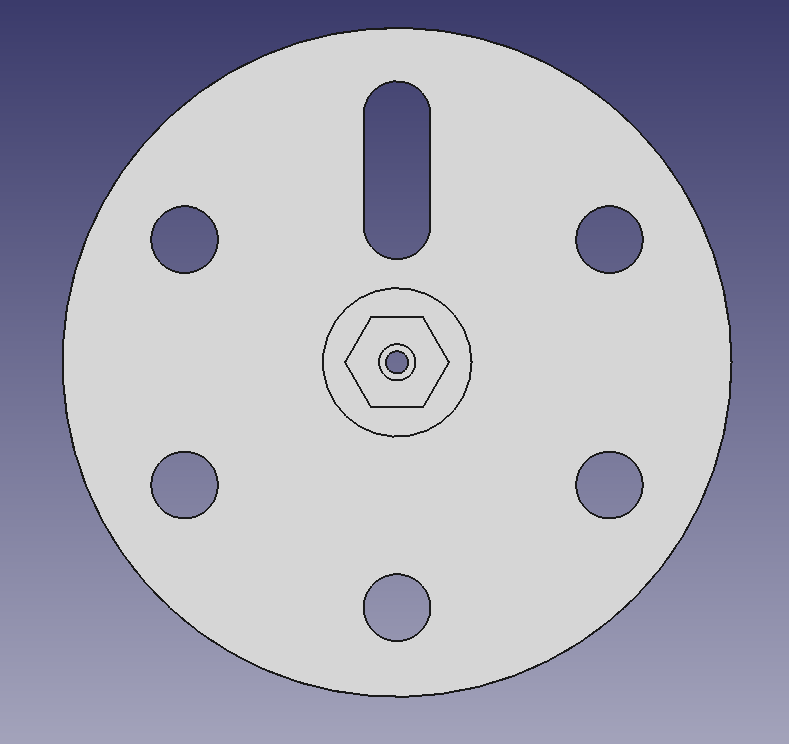
\includegraphics[width=5cm]{img/fly_wheel_side.png}
	\caption{Fly wheel side render view}
	\label{fig:Fly wheel side render view}
\end{figure}

To control the inclination of the body two strategies are taken in to account.
Creating torque by a pendulum or accelerating the flywheel.
In order to experiment with both of them we designed a part to allow
 both configuration by placing weights in different spots, see figure
 \ref{fig:Fly wheel side render view}.

In order to create a configuration with maximum gravitational torque
we have done the following computation. We denote the torque pendulum
torque $\tau$, consider the masses are cylinders of mass $m_{cylinder}$
with radius $r_{cylinder}$ and width $w$ and the radius of the flywheel is $r_{flywheel}$.

Each mass weights:
\[ m_{cylinder} = \rho \cdot w \cdot \pi \cdot r_{cylinder}^2 \]

We neglect the mass of the flywheel structure versus the mass of the cylinders so
all the gravitational torque created by the masses will be compensated with the
opposite weight except for the two masses with different radius.

One of the weight can be placed along a rail. The distance to the center will
vary from $r_{min} = r_{cylinder} + r_{motor-axis} \approx r_{cylinder} $ to $r_{max} = r_{flywheel} - r_{cylinder}$. 

The maximum torque takes place when these two masses are aligned horizontal with respect the ground and the movable weight is at distance $r_{min}$ from the center.

\[ \tau _{max} (r_{cylinder}) =  m_{cylinder} \cdot g \cdot r_{max} -  m_{cylinder} \cdot g \cdot r_{min} =
 m_{cylinder}\cdot g \cdot (r_{flywheel} - 2 \cdot r_{cylinder}) \]

In order to maximize $\tau$ it we first compute the derivative:
\[\frac{\partial \tau _{max} (r_{cylinder})}{\partial r_c} = g \cdot(\frac{\partial m}{\partial r_c} \cdot (r_f - 2 \cdot r_c) -  m_{cylinder} \cdot 2)\]

\[ \frac{\partial  m_{cylinder}}{\partial r_{cylinder}} = 2 \cdot \rho \cdot w \cdot \pi \cdot  r_{cylinder}\]

An make it zero to find the maximum:

\[\frac{\partial \tau _{max} (r_{cylinder})}{\partial r_{cylinder}} = 0\]

Substituting and simplifying we get:

\[\frac{\partial m}{\partial r_{cylinder}} \cdot (r_{flywheel} - 2 \cdot r_{cylinder}) = 
m_{cylinder} \cdot 2 \Rightarrow 2 \cdot \rho \cdot w \cdot \pi \cdot  r_{cylinder}\ \cdot (r_{flywheel} - 2 \cdot r_{cylinder}) = \rho \cdot w \cdot \pi \cdot r_c^2 \cdot 2 \]

\[ \Rightarrow r_c\ \cdot (r_{flywheel} - 2 \cdot r_{cylinder}) =  r_{cylinder}^2 
\Rightarrow (r_{flywheel} - 2 \cdot r_{cylinder}) =  r_{cylinder} 
\Rightarrow \boxed{r_f = 3 \cdot r_{cylinder}}\]


The circumradius $R$ from the center of a regular polygon to one of the vertices is related to the side length $s$ by:

\begin{center}
	\begin{tabular}{ c  c }
		\(\displaystyle R=\frac {s}{2\cdot \sin{\frac {\pi} {n}}} \)
		& 
		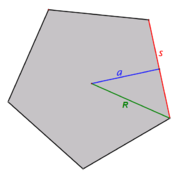
\includegraphics[width=3cm]{img/PolygonParameters.png}
	\end{tabular}
\end{center}

In our case:
\[ R = r_{flywheel} - r_{cylinder}; \]
\[ s = 2 \cdot r_{cylinder}\]

Substituting in the circumradius equation we get n = 6, so we will use up 6 masses in our flywheel.
We will have a variable number of masses $N$ that we will be able to add to
the flywheel as shown in the following table:
\begin{center}
	\begin{tabular}{c | c | c | c }
	 2 & 3 & 4 & 6 \\
	 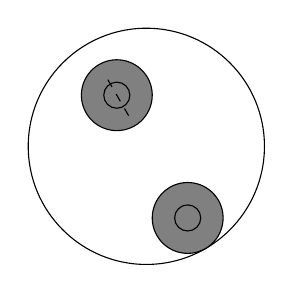
\begin{tikzpicture}[scale=0.5]
		%Circle
			\path node (center) at (0,0) {};
			\draw (center) circle (3);
		%Movable mass
			\draw[rotate=120,fill=gray] (1.5,0) circle (.9) node (moving) [draw,circle]{};
		%Guide
			\draw[dashed,rotate=120] (.9,0) -- (2.1,0);
		%Other masses
			\foreach \i in {2}
			{
				\draw[rotate=60-60*\i,fill=gray] (3-.9,0) circle (.9) node[draw,circle]{};
			}
	\end{tikzpicture}
	
	 & 
	 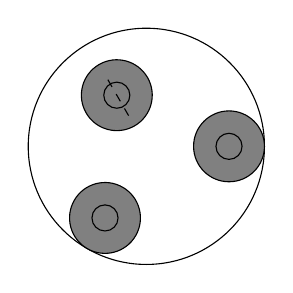
\begin{tikzpicture}[scale=0.5]
		%Circle
			\path node (center) at (0,0) {};
			\draw (center) circle (3);
		%Movable mass
			\draw[rotate=120,fill=gray] (1.5,0) circle (.9) node (moving) [draw,circle]{};
		%Guide
			\draw[dashed,rotate=120] (.9,0) -- (2.1,0);
		%Other masses
			\foreach \i in {1,3}
			{
				\draw[rotate=60-60*\i,fill=gray] (3-.9,0) circle (.9) node[draw,circle]{};
			}
	\end{tikzpicture}
	 & 
	 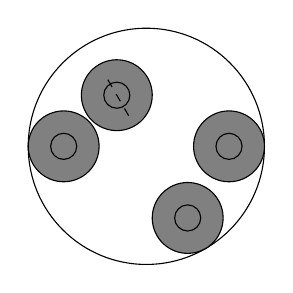
\begin{tikzpicture}[scale=0.5]
		%Circle
			\path node (center) at (0,0) {};
			\draw (center) circle (3);
		%Movable mass
			\draw[rotate=120,fill=gray] (1.5,0) circle (.9) node (moving) [draw,circle]{};
		%Guide
			\draw[dashed,rotate=120] (.9,0) -- (2.1,0);
		%Other masses
			\foreach \i in {1,2,4}
			{
				\draw[rotate=60-60*\i,fill=gray] (3-.9,0) circle (.9) node[draw,circle]{};
			}
	\end{tikzpicture} 
	&
	
	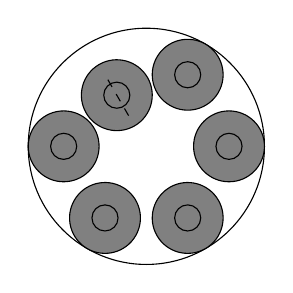
\begin{tikzpicture}[scale=0.5]
		%Circle
			\path node (center) at (0,0) {};
			\draw (center) circle (3);
		%Movable mass
			\draw[rotate=120,fill=gray] (1.5,0) circle (.9) node (moving) [draw,circle]{};
		%Guide
			\draw[dashed,rotate=120] (.9,0) -- (2.1,0);
		%Other masses
			\foreach \i in {1,2,3,4,6}
			{
				\draw[rotate=60-60*\i,fill=gray] (3-.9,0) circle (.9) node[draw,circle]{};
			}
	\end{tikzpicture}
	\\  
	\end{tabular}
	\end{center}

\section{Mechanical analysis} \label{sec: mechanical analysis}
In this section we will analyze and understand the key dynamics of our robot, so we can choose
the design parameters based on performance indicators. All the analysis is made
supposing the inclination of the platform is maintained fixed. As parameters, we have the width of the
flywheel masses $w$, the number of masses $N$, the radius of the flywheel $r_{flywheel}$, and
the radius of the wheels $r_{wheel}$.

\subsection{Inclination control}
In order to keep the inclination of the platform at a certain angle $\phi$ 
we must be able to compensate all the torque being applied to the platform.

\[\ddot{\phi}\cdot I_{platform} = \tau_{platform} \]

Assuming that the platform is well-balanced (the center of masses is located
at the rotation axis by our design restriction) and neglecting the torque generated
by the friction
with air, the sum of all the torques in the motor axis applied to the platform
is equal to the sum of the torque applied by the motors:

\[\tau_{platform} = \sum \tau_{motors}\]

The torque that the motors deliver to the wheels and to the flywheel create
a reaction in the platform in the opposite direction.

\[\tau_{platform} = -\tau_{motor-right-wheel} -\tau_{motor-left-wheel} -\tau_{motor-flywheel} \]

If we want keep the inclination $\phi$, we must be able to cancel $\tau_{platform}$.
Observe that the angular acceleration $\ddot{\phi}$ of the platform is linearly 
dependent with the torque it receives. 
\begin{equation} \label{eq:control equation}
\begin{split}
0 = -\tau_{motor-right-wheel} -\tau_{motor-left-wheel} -\tau_{motor-flywheel} \Rightarrow \\
\tau_{motor-right-wheel} +\tau_{motor-left-wheel} = -\tau_{motor-flywheel}
\end{split}
\end{equation}
In other words, we must overpass the torque of the wheels with the torque of the flywheel
if we want to control the inclination.

\subsection{Wheels torque}
The wheel torque we can induce is limited by the motor specifications.
Note that the maximum torque of the motor is a function of velocity and in particular 
at max speed the torque is zero. See figure \ref{fig: Motor torque} to see the plot of this function.

\[\tau_{motor-wheel} (\omega_{wheel}) \]

\begin{figure}
	\centering
    \begin{tikzpicture}
        %Axis
            \draw[->,thin] (center.center) -- (0,3.5) node[above] {$\tau_{motor}$};
            \draw[->,thin] (center.center) -- (3.5,0) node[right] {$\omega$};
        %Function
            \node (stall) at (0,3) [left]{stall torque};
            \node (maximum) at (3,0) [below]{maximum speed};
            \draw[-] (0,3) -- (3,0);
        \end{tikzpicture}
    \caption{Motor torque.}
	\label{fig: Motor torque}
\end{figure}

We assume that the wheels just roll and do no slip.
The robot is pushed by the wheels that make a force $F_{friction}$ against the ground in the contact point. See figure \ref{fig:Wheel force diagram}.

We can express the torque at the center of the wheel as:
\[\tau_{motor-wheel} + F_{friction} \cdot r_{wheel} = I_{wheel} 
\cdot \dot{\omega}_{wheel} \]
\begin{equation} \label{wheel torque equation}
\tau_{motor-wheel} = I_{wheel} \cdot \dot{w}_{wheel} - F_{friction} \cdot r_{wheel}
\end{equation}
\begin{figure}[ht]
	\centering
	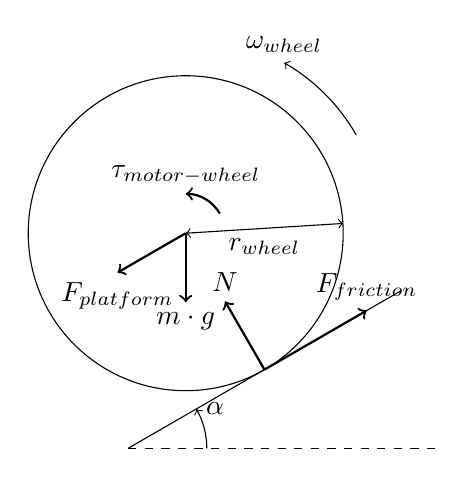
\begin{tikzpicture}
        \path[rotate=30] node (center) at (2,2) {};
        \draw (center) circle (2);
        \draw[rotate=30] (0,0) -- (4,0);
        \draw[dashed] (0,0) -- (4,0);
        \path node[above] (right) at ([shift=({2,0})]center) {};
        \draw[<->] (center.center) -- (right.center)  node[below, midway] {$r_{wheel}$};;
    %Arcs
        \draw[rotate=30, ->] (4.5,2) arc (0:30:2.5) node[above]{$\omega_{wheel}$};
        \draw[rotate=30, ->, thick] (2.5,2) arc (0:60:.5) node[above]{$\tau_{motor-wheel}$};

        \draw[->] (1,0) arc (0:30:1) node[right]{$\alpha$};
    %Forces
        \draw[rotate=30,->,thick] (2,0) -- (3.5,0) node[above]{$F_{friction}$};
        \draw[rotate=30,->,thick] (2,0) -- (2,1) node[above]{$N$};
        \path node[above] (below) at ([shift=({0,-1})]center) {};
    
        \draw[->,thick] (center.center) -- (below.center) node[below]{$m\cdot g$};
        \draw[rotate=30,->,thick] (center.center) -- (1,2) node[below]{$F_{platform}$};
    \end{tikzpicture}
	\caption{Wheel force diagram.}
	\label{fig:Wheel force diagram}
\end{figure}


\subsection{Flywheel torque}
\begin{figure}
	\centering
    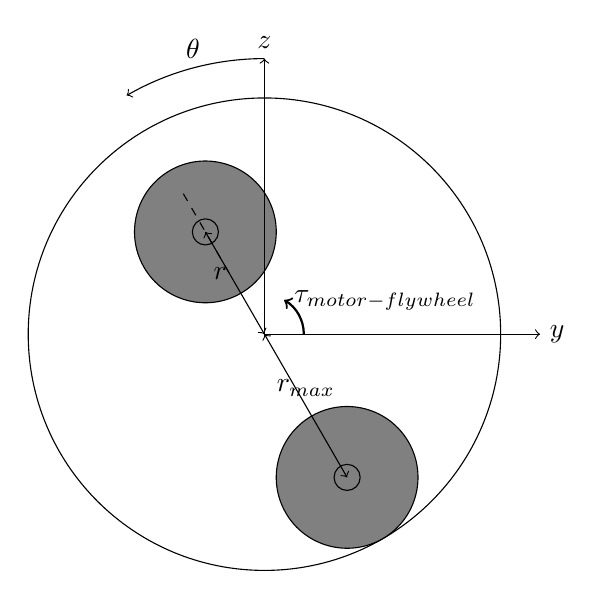
\begin{tikzpicture}
        %Circle
            \path node (center) at (0,0) {};
            \draw (center) circle (3);
        %Arcs
            \draw[->] (0,3.5) arc (90:120:3.5) node[above, midway]{$\theta$};
        %Movable mass
            \draw[rotate=120,fill=gray] (1.5,0) circle (.9) node (moving) [draw,circle]{};
        %Guide
            \draw[dashed,rotate=120] (.9,0) -- (2.1,0);
        %Other masses
            \foreach \i in {2}
            {
                \draw[rotate=60-60* \i,fill=gray] (3-.9,0) circle (.9) node[draw,circle]{};
            }
        %Radius
            \draw[<->] (0,0) -- (moving.center) node[near end, below] {$r$};
            \draw[rotate=-60,<->] (0,0) -- (2.1,0) node[midway, above] {$r_{max}$};
        %Axis
            \draw[->,thin] (center.center) -- (0,3.5) node[above] {$z$};
            \draw[->,thin] (center.center) -- (3.5,0) node[right] {$y$};
        %Motor torque
        \draw[->, thick] (0.5,0) arc (0:60:.5) node[right]{$\tau_{motor-flywheel}$};    
    \end{tikzpicture}
            \caption{Flywheel diagram for $N$ = 2}
	\label{fig:Flywheel force diagram}
\end{figure}

The flywheel torque we can induce is also limited by the motor specifications. 

Assuming a general configuration of the flywheel where the moving mass is at distance $r$ from 
the axis and angle $\theta$, see figure \ref{fig:Flywheel force diagram}, we formulate its torque the following way:
\[
    \tau_{motor-flywheel} + m_{cylinder} \cdot g \cdot (r - r_{max}) \cdot \sin{\theta} = \ddot{\theta}\cdot I_{flywheel}(r)  
\]
\begin{equation}\label{eq: flywheel torque equation}    
    \tau_{motor-flywheel} = \ddot{\theta}\cdot I_{flywheel}(r) + m_{cylinder} \cdot g \cdot (r_{max} - r) \cdot \sin{\theta}  
\end{equation}
Note that in equation \ref{eq: flywheel torque equation} the two terms correspond to the two 
two mechanisms: acceleration of the flywheel and position of the pendulum.

\subsection{Maximum speed, acceleration and terrain inclination}
In this subsection we would like to study the maximum speed and acceleration the robot may
obtain in straight direction and the maximum terrain inclination it can stand on $\alpha$.

We will assume both wheels turn at the same speed, have the same $F_{friction}$ and the same $\tau_{wheel}$:
\[ \omega_{wheel-left} = \omega_{wheel-right} = \omega_{wheel} \]
\begin{figure}
	\centering
	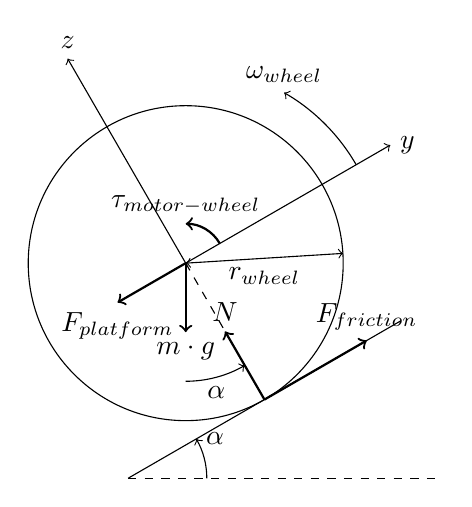
\begin{tikzpicture}
        \path[rotate=30] node (center) at (2,2) {};
        \draw (center) circle (2);
        \draw[rotate=30] (0,0) -- (4,0);
        \draw[dashed] (0,0) -- (4,0);
        \path node[above] (right) at ([shift=({2,0})]center) {};
        \draw[<->] (center.center) -- (right.center)  node[below, midway] {$r_{wheel}$};;
    %Arcs
        \draw[rotate=30, ->] (4.5,2) arc (0:30:2.5) node[above]{$\omega_{wheel}$};
        \draw[rotate=30, ->, thick] (2.5,2) arc (0:60:.5) node[above]{$\tau_{motor-wheel}$};

        \draw[->] (1,0) arc (0:30:1) node[right]{$\alpha$};
        \draw[rotate=30,<-] (2,.5) arc (270:240:1.5) node[below, midway]{$\alpha$};
    %Forces
        \draw[rotate=30,->,thick] (2,0) -- (3.5,0) node[above]{$F_{friction}$};
        \draw[rotate=30,->,thick] (2,0) -- (2,1) node[above]{$N$};
        \path node[above] (below) at ([shift=({0,-1})]center) {};
    
        \draw[->,thick] (center.center) -- (below.center) node[below]{$m\cdot g$};
        \draw[rotate=30,->,thick] (center.center) -- (1,2) node[below]{$F_{platform}$};
    %Axis
        \draw[->,thin][rotate=30] (center.center) -- (2,5) node[above] {$z$};
        \draw[->,thin][rotate=30] (center.center) -- (5,2) node[right] {$y$};
        \draw[dashed][rotate=30] (center.center) -- (2,1);

    \end{tikzpicture}
    \caption{Wheel forward force diagram.}
    \label{fig:Wheel forward force diagram}
\end{figure}

Applying Newton's first law in the y-axis of figure \ref{fig:Wheel forward force diagram}:
\[\ddot{y}\cdot m_{total} = 2 \cdot F_{friction} - m_{total} \cdot g \cdot sin(\alpha)\]
Substituting $F_{friction}$ taking in to account equation \ref{wheel torque equation}:
\[\ddot{y}\cdot m_{total} = 2 \cdot \frac{I_{wheel} \cdot \dot{w}_{wheel}-\tau_{motor-wheel}}{r_{wheel}} - m_{total} \cdot g \cdot sin(\alpha)\]
Using equation \ref{eq:control equation}:
\begin{equation}\label{eq of acceleration}
    \Rightarrow  \ddot{y}\cdot m_{total} = \frac{2\cdot I_{wheel} \cdot \dot{w}_{wheel}}{r_{wheel}} + \frac{\tau_{motor-flywheel}}{r_{wheel}} - m_{total} \cdot g \cdot sin(\alpha)
\end{equation}
We will now study different cases to better understand this equation.

\subsubsection{Speed and acceleration with no terrain inclination ($\alpha = 0$)}
The objective here is to obtain the maximum speed and acceleration we can get starting from rest in a plain surface.

The equation we get by substituting $\alpha = 0$ in equation \ref{eq of acceleration}:
\[\ddot{y}\cdot m_{total} = \frac{\tau_{motor-flywheel}}{r_{wheel}} +\frac{2\cdot I_{wheel} \cdot  \dot{w}_{wheel}}{r_{wheel}}\]

Substituting equation \ref{eq: flywheel torque equation}:
\begin{equation}\label{eq: no inclintation}
    \ddot{y}\cdot m_{total} = \frac{\ddot{\theta}\cdot I_{flywheel}(r) +
    m_{cylinder} \cdot  g \cdot  (r_{max} - r) \cdot  \sin{\theta}}{r_{wheel}} +\frac{2\cdot I_{wheel} \cdot  \dot{\omega}_{wheel}}{r_{wheel}}
\end{equation}


We will now split the study in two cases:
\begin{enumerate}
    \item \textbf{Flywheel case:} $r$ is fixed to $r = r_{max}$ 
    
    Then:  
    \[\ddot{y}\cdot m_{total} = - \frac{\ddot{\theta}\cdot I_{flywheel}(r_{max})}
    {r_{wheel}} + \frac{2\cdot I_{wheel} \cdot  \dot{\omega}_{wheel}}{r_{wheel}}\]

    Taking in to account the following relation:
    \begin{equation} \label{eq: angular velocity}
        -\omega_{wheel} \cdot  r_{wheel} = \dot{y} \Rightarrow  -\dot{\omega}_{wheel} \cdot  r_{wheel} = \ddot{y}  
    \end{equation}

    Substituting in equation \ref{eq: no inclintation}:
    \[-\dot{\omega}_{wheel} \cdot  r_{wheel}\cdot m_{total} = \frac{\ddot{\theta}\cdot I_{flywheel}}
    {r_{wheel}} + \frac{2\cdot I_{wheel} \cdot  \dot{\omega}_{wheel}}{r_{wheel}} \]

    \[-\dot{\omega}_{wheel} \cdot (r_{wheel}\cdot m_{total} +  \frac{2\cdot I_{wheel} }{r_{wheel}}) = 
    \frac{\ddot{\theta}\cdot I_{flywheel}}{r_{wheel}}\]


    We now define R as a non dimensional constant being the quotient between $\dot{w}_{wheel}$ and $-\ddot{\theta}$.

    \begin{equation}\label{eq: R definition}
        R = \frac{\dot{\omega}_{wheel}}{-\ddot{\theta}} = 
    \frac{I_{flywheel}}
    {r_{wheel}^2\cdot m_{total} +  2\cdot I_{wheel}}
    \end{equation}

    The moments of inertia are:
    \[I_{wheel} \approx \frac{1}{2} \cdot m_{wheel} \cdot  r_{wheel}^2\]
    \[I_{flywheel} \approx N \cdot  m_{cylinder} \cdot  r_{max}^2\]

    Substituting those in equation \ref{eq: R definition} we get:
    \[R \approx
    \frac{ N \cdot  m_{cylinder} \cdot  r_{max}^2}
    {r_{wheel}^2\cdot m_{total} +  2\cdot I_{wheel}} < 1 \] 

    We can see that R will always be smaller than 1 because $N \cdot  m_{cylinder} < m_{total} $ and $r_{max} < r_{wheel}$.
    
    This means that the maximum acceleration of the wheels will be limited by the acceleration of the flywheel. The same is true for the speed.

    In  order to get the forward acceleration we can use equation \ref{eq: angular velocity}
    \[\ddot{y} = -\dot{\omega}_{wheel} \cdot  r_{wheel} = R \cdot  \ddot{\theta} \cdot  r_{wheel}\]
    And using equation \ref{eq: flywheel torque equation} we get that the maximum is:

    \[\tau_{motor} (\omega) = \ddot{\theta}\cdot I_{flywheel}(r) \Rightarrow \ddot{\theta} = \frac{\tau_{motor} (\dot{\theta})}{I_{flywheel}(r)} \]

    \[\ddot{y}_{max} = R \cdot  \frac{\tau_{motor} (\dot{\theta})}{I_{flywheel}(r)} \cdot  r_{wheel}\]

    \[\Rightarrow \ddot{y}_{max} =     \frac{I_{flywheel}}
    {r_{wheel}^2\cdot m_{total} +  2\cdot I_{wheel}}  \cdot  \frac{\tau_{motor} (\dot{\theta})}{I_{flywheel}(r)} \cdot  r_{wheel}\]
    \begin{equation}        
        \boxed{\ddot{y}_{max} = \frac{\tau_{motor}(\dot{\theta})\cdot r_{wheel} }
        {r_{wheel}^2\cdot m_{total} +  2\cdot I_{wheel}}}
        \label{maximum acceleration flywheel}
    \end{equation}
    In order to compute the maximum speed we assume that the initial conditions are $\dot{\theta} = 0$ and 
    $\omega_{wheel}=0$

    \[\omega_{wheel-max} = \int_{t=0}^{t=t_{max}} \dot{\omega}_{wheel} \cdot  dt\]

    Now we will proceed to do a change of variables in the integral.

    \[
    \frac{\partial \dot{\theta}}{\partial t} = \ddot{\theta} \Rightarrow dt = \frac{d\dot{\theta}}{\ddot{\theta}}
    \]
    
    \[\omega_{wheel-max} = \int_{\dot{\theta}=0}^{\dot{\theta}=\dot{\theta}_{max}} \frac{\dot{\omega}_{wheel}}{\ddot{\theta}} \cdot  d\dot{\theta} = 
    \int_{\dot{\theta}=0}^{\dot{\theta}=\dot{\theta}_{max}} -R \cdot  d\dot{\theta} = - R \cdot  \dot{\theta}_{max}
    \]
    \begin{equation}
        \boxed{\dot{y}_{max} = r_{wheel} \cdot  R \cdot  \dot{\theta}_{max}}
        \label{Maximum speed flywheel}
    \end{equation}
    And $\dot{\theta}_{max}$ is a limitation imposed by the motor specifications. Note that this is the maximum speed
    we can get using the flywheel system starting from rest.


    \item \textbf{Pendulum:} $\dot{\theta} = 0$, and $r$ is fixed to $r = r_{min}$
    
    Using equation \ref{eq: no inclintation} and $\ddot{\theta} = 0$
    \[\ddot{y}\cdot m_{total} = \frac{m_{cylinder} \cdot  g \cdot  (r_{max} - r_{min}) \cdot  \sin{\theta}}{r_{wheel}} +\frac{2\cdot I_{wheel} \cdot  \dot{w}_{wheel}}{r_{wheel}}\]
    Multiplying by $r_{wheel}$ both sides of the equation we get:
    \[\ddot{y}\cdot m_{total} \cdot  r_{wheel} = m_{cylinder} \cdot  g \cdot  (r_{max}-r_{min}) \cdot  \sin{\theta} + 2\cdot I_{wheel} \cdot  \dot{w}_{wheel}\]
    And using $\dot{w}_{wheel} = -\frac{\ddot{y}}{r_{wheel}}$
    \[\ddot{y}\cdot m_{total} \cdot  r_{wheel} + 2\cdot  I_{wheel} \cdot  \frac{\ddot{y}}{r_{wheel}} = m_{cylinder} \cdot  g \cdot  (r_{max}-r) \cdot  \sin{\theta} \]
    With some manipulation:
    \[\ddot{y}  = \frac{m_{cylinder} \cdot  g \cdot  (r_{max}-r_{min}) \cdot  \sin{\theta}}{m_{total} \cdot  r_{wheel} + \frac{2\cdot I_{wheel}}{r_{wheel}} }  \]
    Which is maximum when $\sin{\theta}=1$
    \begin{equation}
        \boxed{ \ddot{y}_{max}  = \frac{m_{cylinder} \cdot  g \cdot  (r_{max}-r_{min}) \cdot}{m_{total} \cdot  r_{wheel} + \frac{2\cdot I_{wheel}}{r_{wheel}} } }
        \label{maximum acceleration pendulum}
    \end{equation}
    Since the maximum acceleration obtained is constant, the speed could increase without limit. To get a meaningful estimation of the maximum speed,
    we will take into account the air friction that becomes more and more important as the speed increases.
    
    \[F_{drag} = \frac{1}{2}\cdot \rho\cdot C_D \cdot  A \cdot  \dot{y}^2 \]

    Adding this term to equation \ref{eq of acceleration} we get:
    \[  \ddot{y}\cdot m_{total} = \frac{2\cdot I_{wheel} \cdot  \dot{w}_{wheel}}{r_{wheel}} + \frac{\tau_{motor-flywheel}}{r_{wheel}} - m_{total} \cdot  g \cdot  sin(\alpha) - F_{drag} \]
    And making $\ddot{y} = 0$ and $\alpha = 0$.
    \[  F_{drag} = \frac{\tau_{motor-flywheel}}{r_{wheel}}\]

    \[\frac{1}{2}\cdot \rho\cdot C_D \cdot  A \cdot  \dot{y}^2 = m_{cylinder} \cdot  g \cdot  (r_{max} - r_{min})\cdot sin(\theta) / r_{wheel} \]
    The maximum $\dot{y}$ is then obtained when $\theta=\frac{\pi}{2}$:
    \begin{equation*}
        \dot{y}_{max} = \sqrt{\frac{2\cdot m_{cylinder} \cdot  g \cdot  (r_{max} - r_{min})}{\rho\cdot C_D \cdot  A \cdot  r_{wheel}} }
    \end{equation*}

    We will pick $C_D=1$, $\rho=1.2 kg/m^3$ and $A=0.01 m^2$ for our computations.

    Also, note that the speed is also limited by maximum speed a motor can get
    $\dot{\theta}_{max}$.
    \begin{equation}
        \boxed{\dot{y}_{max} = min(\dot{\theta}_{max}\cdot r_{wheel}, \sqrt{\frac{2\cdot m_{cylinder} \cdot  g \cdot  (r_{max} - r_{min})}{\rho\cdot C_D \cdot  A \cdot  r_{wheel}} })}
        \label{maximum speed pendulum}
    \end{equation}


\end{enumerate}
\subsubsection{Terrain inclination ($\alpha > 0$)}
The goal of this subsection is to study which is the maximum terrain inclination $\alpha_{max}$ 
on which the robot can stay, standing still without rolling down.

Substituting $\ddot{y}=0$ and $\dot{\omega}_{wheel} = 0$ in equation \ref{eq of acceleration}
\[0 = \frac{\tau_{motor-flywheel}}{r_{wheel}} - m_{total} \cdot  g \cdot  sin(\alpha)\]
\[m_{total} \cdot  g \cdot  sin(\alpha) = \frac{\tau_{motor-flywheel}}{r_{wheel}} \]
\[sin(\alpha) = min(1,\frac{\tau_{motor-flywheel}}{m_{total} \cdot  g \cdot  r_{wheel}}) \]

Substituting equation \ref{eq: flywheel torque equation}
\[sin(\alpha) = min(1,\frac{\ddot{\theta}\cdot I_{flywheel}(r) + m_{cylinder} \cdot  g \cdot  (r_{max} - r) \cdot  \sin{\theta}}{m_{total} \cdot  g \cdot  r_{wheel}}) \]


We are going to distinguish the same two cases as in the previous section:
\begin{enumerate}
    \item Flywheel case: $r$ is fixed to $r = r_{max}$
    The maximum inclination at a certain moment:
    \begin{equation}\label{Maximum angle using flywheel system}
        \boxed{sin(\alpha_{max}) = min(1,\frac{\ddot{\theta}\cdot I_{flywheel}}{m_{total} \cdot  g \cdot  r_{wheel}}) = min(1,\frac{\tau_{motor-flywheel}(\dot{\theta})}{m_{total} \cdot  g \cdot  r_{wheel}})}
    \end{equation}


    This angle doesn't give us a lot of information because it may not be fulfilled in a 
    permanent state.
    
    \item Pendulum: $\dot{\theta} = 0$, and $r$ is fixed to $r = r_{min}$
    \[sin(\alpha) = \frac{min(\tau_{motor-flywheel},m_{cylinder} \cdot  g \cdot  (r_{max} - r_{min}) \cdot  \sin{\theta})}{m_{total} \cdot  g \cdot  r_{wheel}} \]
    Which is maximum when $\sin{\theta} = 1$
    \begin{equation}\label{Maximum angle using pendulum system}
        \boxed{sin(\alpha_{max}) = \frac{min(\tau_{motor-flywheel},m_{cylinder} \cdot  g \cdot  (r_{max} - r_{min}))}{m_{total} \cdot  g \cdot  r_{wheel}}}
    \end{equation}
    Note that the $sin(\alpha_{max})$ will not be more than 1.
\end{enumerate}


\section{Optimization}
In this section we select which parameters are going to be used when building our robot.

\subsection{Minimum section in the section of the flywheel}
We wil place our flywheel in a hole on our robot. We will now compute the minimum section in hole so it doesn't bend. See figure \ref{fig:Flywheel hole diagram}.

\begin{figure}[ht]
	\centering
	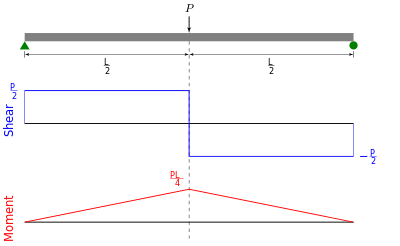
\includegraphics[width=10cm]{img/Shear_Moment_Diagram.png}
	\caption{Bendig moment diagram}
	\label{fig:Bendig moment diagram}
\end{figure}
The maximum bending moment is at the flywheel section:
\[M_y = \frac{P * L}{4}\]
Where P is the weight of the robot and L is the distance between the two wheels.

\[I_y = \frac{2*b*h^3}{12}=\frac{b*h^3}{6}\]
\[\sigma=\frac{M_y}{I_y}*\frac{h}{2} = \frac{P*L}{48*b*h^2}\]
We are planning to build our body structure with plastic:
\[\sigma_{plastic} = 4MPa = 4E6Pa\]
We will impose the relation:
\[b = h\]
And set a target P of $2000N$ and a maximum length of $0.5m$
\[\sigma_{plastic} = 4E6Pa = \frac{P*L}{48*b*h^2} = \frac{1000}{48*b^3} \]
Therefore:
\[b = \sqrt[3]{\frac{1000}{48*4E6}} = 1,277182 m\]
We will use b=10mm and h=10mm from now on. Which is far more than what we need.


\subsection{Restrictions}
The first restrictions is due to the initial design requirements. The other three are somehow arbitrary but will help us to reduce the size of the robot.
\begin{enumerate}
\item We wil place our flywheel in a hole on our robot. We don't want to touch the ground in any configuration so:
\begin{figure}[ht]
	\centering
	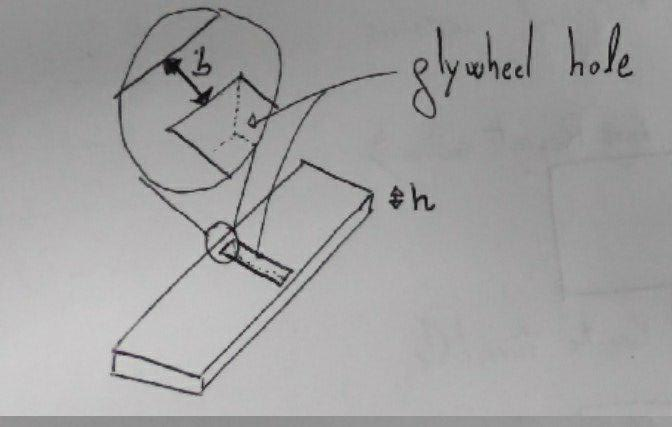
\includegraphics[width=5cm]{img/flywheel_hole.jpg}
	\caption{Flywheel hole diagram}
	\label{fig:Flywheel hole diagram}
\end{figure}
\[r_{wheel}> \sqrt{(r_{flywheel} + b)^2+(\frac{h}{2})^2}\]
\item Being able  to insert the robot in to a wheel of diameter 0.5m so:
\begin{figure}[ht]
	\centering
	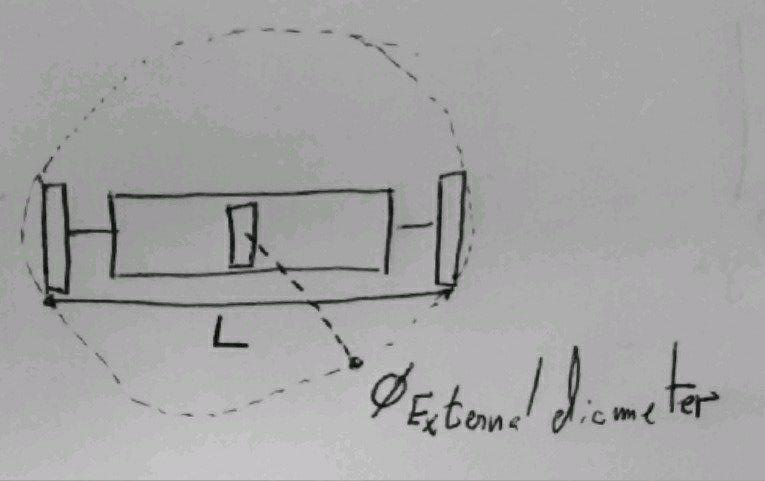
\includegraphics[width=5cm]{img/external_diameter.jpg}
	\caption{External diameter diagram}
	\label{fig:External diameter diagram}
\end{figure}
\[0.25 m > \sqrt{r_{wheel}^2 + L^2/4}\]
\item We can place all electronic the devices:
\[L > 0.3m + w \]
\item Maximum weight of the robot: 5kg
\end{enumerate}

\subsection{Requirements}
Based on the mechanical analysis we have set some requirements that we would like our robot to fullfil:
\textbf{Flywheel mode}
\begin{enumerate}
	\item $\dot{y}_{max}$ (equation \ref{Maximum speed flywheel}) $> 0.1m/s$
	\item $\ddot{y}_{max}$ (equation \ref{maximum acceleration flywheel})> $1m/s^2$
	\item $sin(\alpha_{max})$ (equation \ref{Maximum angle using flywheel system}) $> 0.2$
\end{enumerate}
\textbf{Pendulum mode}
\begin{enumerate}
	\item $\dot{y}_{max}$ (equation \ref{maximum speed pendulum}) $> 1m/s$
	\item $\ddot{y}_{max}$ (equation \ref{maximum acceleration pendulum}) $>0.1m/s^2$
	\item $sin(\alpha_{max})$ (equation \ref{Maximum angle using pendulum system}) $> 0.02$
\end{enumerate}
	


\subsection{Cost function}
Apparat from fulfilling the requirements we will try to minimize a cost function.

We will maximize the maximum sinus in the pendulum mode 
(equation \ref{Maximum angle using pendulum system}) because
it give the robot the capacity to deliver force in a permanent state.

We will also maximize the square of the max speed the robot can achieve
in flywheel mode (equation \ref{Maximum speed flywheel}) because it is
proportional to the energy the robot can deliver using the flywheel at a certain moment.

\begin{equation}
	cost(r_{flywheel},r_{wheel},w,N) = - sin(\alpha_{max})_{pendulum} -\dot{y}^2_{max-flywheel}
	\label{eq: cost}
\end{equation}
\begin{equation*}
	m_{cylinder} = \rho * w * \pi * (\frac{r_{flywheel}}{3})^2
\end{equation*}
\begin{equation*}
	sin(\alpha_{max})_{pendulum} = \frac{m_{cylinder} \cdot  (r_{max} - r_{min})}{m_{total} \cdot r_{wheel}} = \frac{m_{cylinder} \cdot  (\frac{r_{flywheel}}{3})}{(m_{rest} + N \cdot m_{cylinder})\cdot r_{wheel}} 	
\end{equation*}
\begin{equation*}
	\dot{y}_{max} = r_{wheel} \cdot  R \cdot  \dot{\theta}_{max} =r_{wheel} \cdot  \frac{ N \cdot  m_{cylinder} \cdot  (\frac{2\cdot r_{flywheel}}{3})^2}
    {r_{wheel}^2\cdot (m_{rest} + N \cdot m_{cylinder}) +  2\cdot I_{wheel}} \cdot  \dot{\theta}_{max}
\end{equation*}

\subsection{Results}
Our procedure has been making a grid with the four parameters of the robot 
design: $w$ (width of the cylinders), $N$(number of cylinders), $r_{wheel}$ and $r_{flywheel}$.
We have fixed $r_{flywheel}$, iterated over the other three variables and keeped the best parameters to reduce our cost function.


\begin{figure}[H]
	\centering
	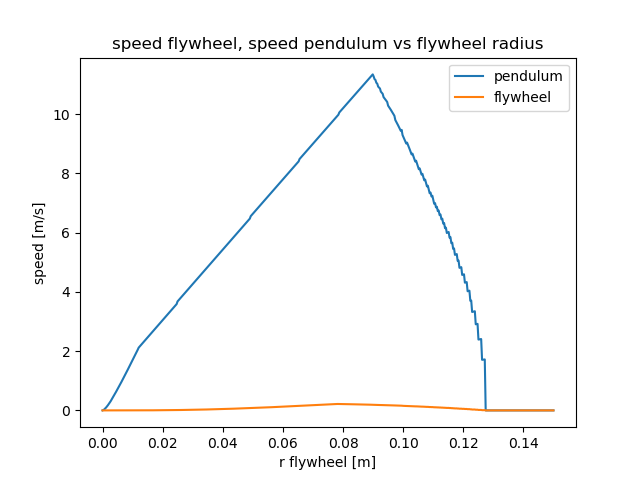
\includegraphics[width=10cm]{img/optimization/speed.png}
	\caption{Plot of the equations \ref{Maximum speed flywheel} and \ref{maximum speed pendulum} at the parameters that minimize the cost function and fullfil the requirements and restrictions}
	\label{fig:Speed plot}
\end{figure}

\begin{figure}[H]
	\centering
	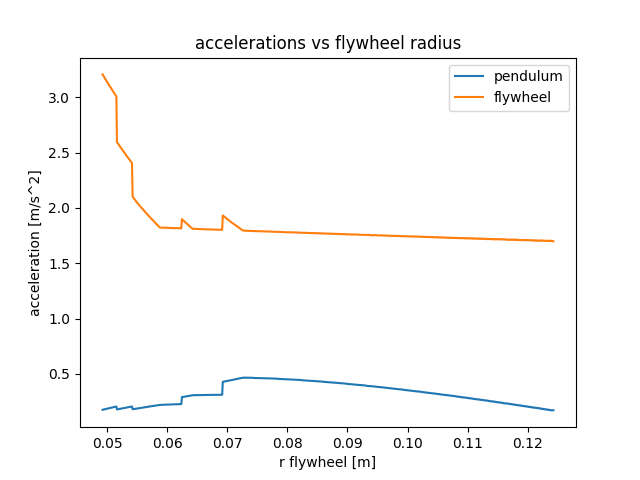
\includegraphics[width=10cm]{img/optimization/acceleration.png}
	\caption{Plot of the equations \ref{maximum acceleration flywheel} and \ref{maximum acceleration pendulum} at the parameters that minimize the cost and fullfil the requirements and restrictions}
	\label{fig:Speed plot}
\end{figure}

\begin{figure}[H]
	\centering
	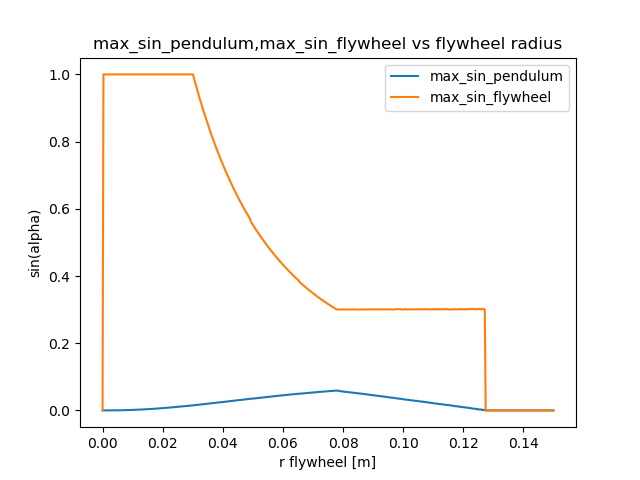
\includegraphics[width=10cm]{img/optimization/sin.png}
	\caption{Plot of the equations \ref{Maximum angle using flywheel system} and \ref{Maximum angle using pendulum system} at the parameters that minimize the cost and fullfil the requirements and restrictions}
	\label{fig:Sinus plot}
\end{figure}

\begin{figure}[H]
	\centering
	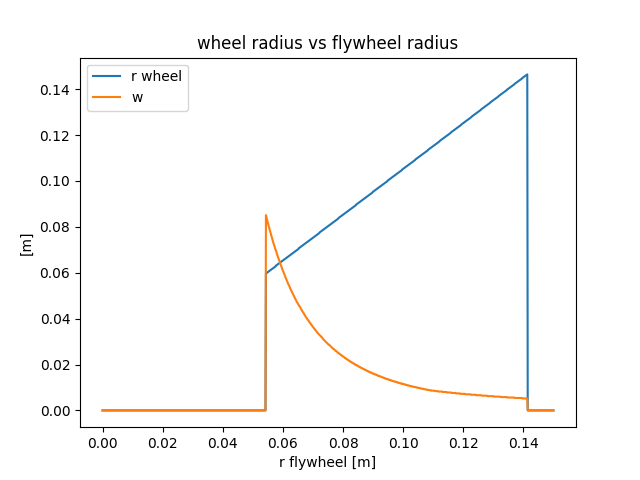
\includegraphics[width=10cm]{img/optimization/parameters.png}
	\caption{Plot of the parameters that minimize the cost function.}
	\label{fig:Parameters plot}
\end{figure}

\begin{figure}[H]
	\centering
	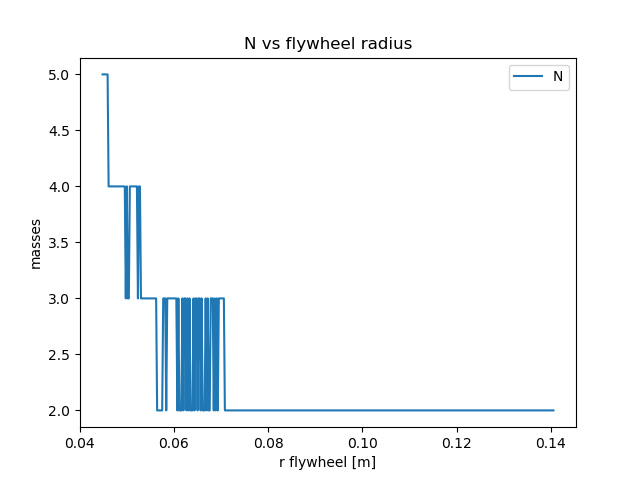
\includegraphics[width=10cm]{img/optimization/N.png}
	\caption{Plot of the N that minimize the cost function.}
	\label{fig:Parameters plot}
\end{figure}

\begin{figure}[H]
	\centering
	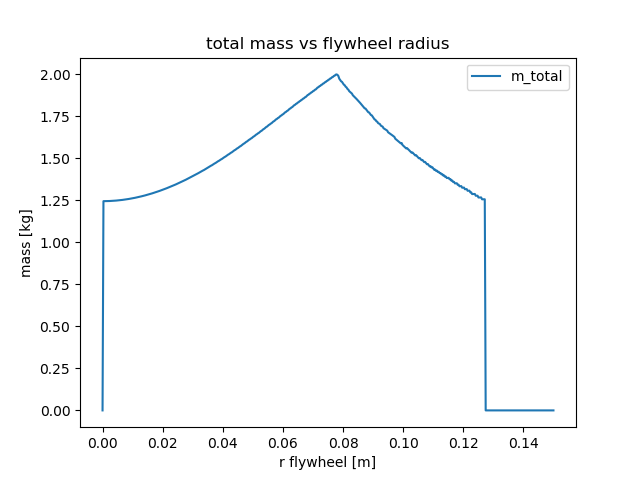
\includegraphics[width=10cm]{img/optimization/mass.png}
	\caption{Plot of the mass for each configuration.}
	\label{fig:Mass plot}
\end{figure}

%\begin{figure}[H]
%	\centering
%	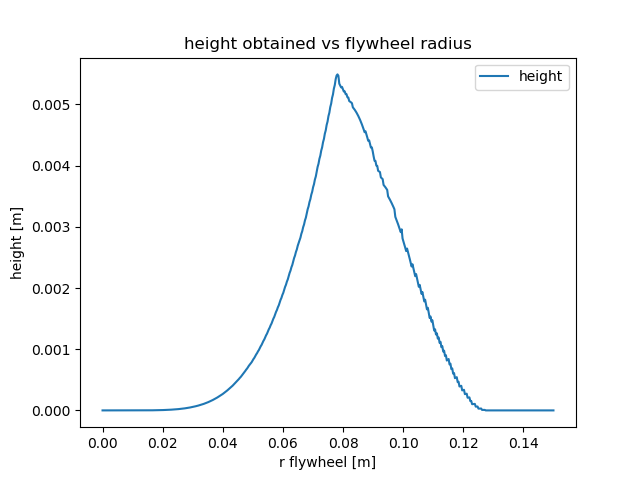
\includegraphics[width=10cm]{img/optimization/height.png}
%	\caption{Plot of the equation \ref{Maximum height} for each configuration.}
%	\label{fig:Mass plot}
%\end{figure}

\begin{figure}[H]
	\centering
	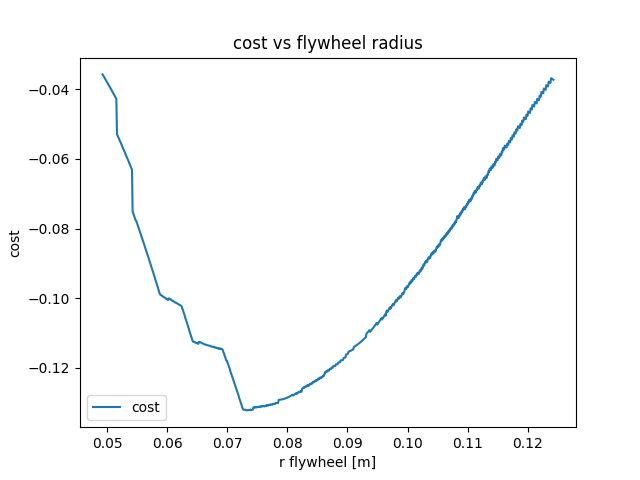
\includegraphics[width=10cm]{img/optimization/cost.png}
	\caption{Plot of the equation \ref{eq: cost} for each configuration.}
	\label{fig:Mass plot}
\end{figure}

Our selected parameters are:
\begin{center}
	\begin{tabular}{ |c|c|c|c| } 
	 \hline
	 $r_{flywheel}$ & $r_{wheel}$ & $w$ & $N$\\
	 \hline 
	 8cm & 10cm & 5cm & 2 \\ 
	 \hline
	\end{tabular}
\end{center}

With this parameters we get the following specifications:
\begin{center}
	\begin{tabular}{ |c|c| } 
	 \hline
	 Total mass & 2,91kg\\
	 \hline
	 \textbf{Pendulum} \\
	 \hline
	 Maximum sinus & 0,042\\
	 \hline
	 Maximum speed horizontal & 1,84 $m/s$\\
	 \hline
	 Maximum acceleration horizontal & 0,38 $m/s^2$\\
	 \hline
	 \textbf{Flywheel} \\
	 \hline
	 Maximum sinus & 0,171\\
	 \hline
	 Maximum speed horizontal & 0,24 $m/s$\\
	 \hline
	 Maximum acceleration horizontal & 1.52 $m/s^2$\\
	 \hline
	\end{tabular}
\end{center}
\section{Flywheel study}

\subsection{System of differential equations}
As described in figure \ref{fig:Flywheel force diagram} we will use two variables to describe the flywheel position: $r$, $\theta$ 
We will use the change of variables $\alpha =\pi/2 - \theta$

Using equation \ref{flywheel equation}:
\[\tau_{flywheel} = \ddot{\theta}*I_{flywheel}(r) + m_{cylinder} * g * (r - r_{max}) * \sin{\theta}\]
And that:
\[\ddot{r} * m = -m * g * sin(\pi/2-\theta) + F_{friction}\]
\[F_{friction} = F_{normal} * \mu\]
\[F_{normal} = -m * g * cos(\pi/2-\theta)\]


\end{document}          
